% beautiful title slides in Beamer
% Model 5
% latex-beamer.com

\documentclass[aspectratio=169]{beamer}

% Remove navigation bar
\setbeamertemplate{navigation symbols}{}

% Tikz package
\usepackage{tikz}
\usetikzlibrary{positioning}
\titlegraphic{
    
\includegraphics[width=2cm]{images/freyja.png}
}

\usepackage[spanish]{babel}
\usepackage{listings}
\usetheme{Boadilla}

\begin{document}
	
	\author{María San José Seco \href{https://github.com/drkrysSrng/freyja}{@drkrysSrng/freyja}} 
	\date{\today} 

	\begin{frame}[plain]
	
	%%%%%%%% Title slide details %%%%%%%%%%%%%%


% Background Image
\newcommand{\myBackround}
{
    
\includegraphics[width=\paperwidth]{images/Background 5.png}
}

% Title
\newcommand{\myTitle}
{
    Estudio práctico de técnicas de ofuscación y contramedidas aplciables
}


% Author
\newcommand{\myAuthor}   
{
    María San José Seco \href{https://github.com/drkrysSrng/freyja}{@drkrysSrng/freyja}
}

% Affiliation
\newcommand{\myAffiliate}
{
    Universidad Católica de Murcia\\
    ENIIT - Campus Internacional de Ciberseguridad
}

% Presentation Date
\newcommand{\myDate}   
{
    \today
}

% Logo 1
\newcommand{\myLogoA}   
{
    
\includegraphics[width=2cm]{images/logo.png}
}

% Logo 2
\newcommand{\myLogoB}   
{
    
\includegraphics[width=5cm]{images/logo_uni.png}
}
%%%%%%%%%%%%%%%%%%%%%%%%%%%%%%%%%%%%


%%%%%%%%%% Title slide code %%%%%%%%%%%
\begin{tikzpicture}[remember picture,overlay]

% Background image
\node[above right,inner sep=0pt] at (current page.south west)
    {
        \myBackround
    };
    
% Title & Subtitle
\node
[
    above=0.5cm,
    align=center,
    fill=black!70,
    text=white,
    rounded corners,
    inner xsep=15pt,
    inner ysep=10pt, 
    minimum width=0.7\textwidth,
    text width=0.6\textwidth
] (title) at (current page.center)
{
    \normalsize \myTitle  
};

% Author 
\node[ below=0.5cm] (author) at (title.south){\myAuthor};

% Author 
\node[ below=0.1cm] (affiliate) at (author.south){\small \myAffiliate};

% Date
\node[below=0.25cm] (date) at (affiliate.south){\large \myDate};

% Logo A
\node
[
    below right =0.25cm and 7.5cm
] at (current page.north west)
{
    \myLogoA
};

% Logo B
\node
[
    below left =0.25cm and 0.5cm
] at (current page.north east)
{
    \myLogoB
};

\end{tikzpicture}
	    
	\end{frame}

	

	\frame{\frametitle{Table of contents}\tableofcontents} 

	
	\begin{frame}{Introducción}
	 \section{Introducción}
		Uso de la ofuscación durante la historia;
		\begin{itemize}
			\item Proteger la propiedad intelectual o intercambiar secretos
			\item Evasión de antivirus, sandboxes, strings por reglas YARA y Analistas de Malware
		\end{itemize}
		\end{frame}
	
    \begin{frame}{Tipos de ofuscación}
    \section{Tipos de ofuscación}
	  	\begin{itemize}
	  		\item \textbf{Packing} Epaquetar un ejecutable dentro de otro encriptado. Ejecución en memoria.
	  		\item \textbf{Inserción de código basura:} Inserción de código sin funcionalidad.
  			\item \textbf{XOR:} Ofuscar variables ya que xoreando una variable consigo misma da resultado 0.
  			\item \textbf{Reasignamiento de registros:} Copias de parámetros.
  			\item \textbf{Sustitución de instrucciones:} Reemplazar operaciones por otras.
  			\item \textbf{Base64:} Ofuscación cadenas de texto.
  			\item \textbf{Transposición de código:} Se cambian las instrucciones de lugar.
  			\item \textbf{Integración de código:} Infección de otros binarios o ficheros con malware encriptado.
  			\item \textbf{Expreciones MBA:} Polinomios y operadores booleanos que sustituyen expresiones por otras equivalentes.
  			\item \textbf{Expresiones Opacas:} Expresiones que siempre son Verdadero o Falso pero sólo en tiempo de ejecución.
  			
  		\end{itemize}
	   \end{frame}

    \begin{frame}{Enriptación, Compresión y Metamorfismo}
    \section{Enriptación, Compresión y Metamorfismo}
    Se ha avanzado mucho, de modo que además de ofuscarse, el malware también se comprime y encripta.
  	  	\begin{itemize}
  	  		\item Oligomorfismo donde la parte viral está encriptada.
  	  		\item Polimorfismo, donde hay ofuscación y encriptación. Primer malware poligomórfico, encontrado fue Luna, desarrollado por Bumblebee en el año 1999.
  	  		\item Metamorfismo, variaciones de ofuscación con muchas subrutinas posibles.
  	  		\item Motor metamórfico, responsable de las técnicas de evasión.    			
   		\end{itemize}
	\end{frame}
	
	\begin{frame}{Motor metamórfico}
   	\subsection{Motor metamórfico}
		\begin{itemize}
			\item \textbf{Dissasembler} Convierte el código binario en ensamblador.    	
			\item \textbf{Shrinker} Elimina código basura.
			\item \textbf{Permutor} Ofuscación con permutaciones y subrutinas.
			\item \textbf{Expander} Sustituye instrucciones por equivalentes.
			\item \textbf{Assembler} Convierte el código ensamblador en binario.
			\item \textbf{Viral Code} Contiene las instrucciones del código malicioso que estarán en todas las permutaciones del malware.	
		\end{itemize}
	   	   	
	\end{frame}
	\begin{frame}{Motor metamórfico}
	\subsection{Motor metamórfico}
		\begin{figure}[H]
			\centering
			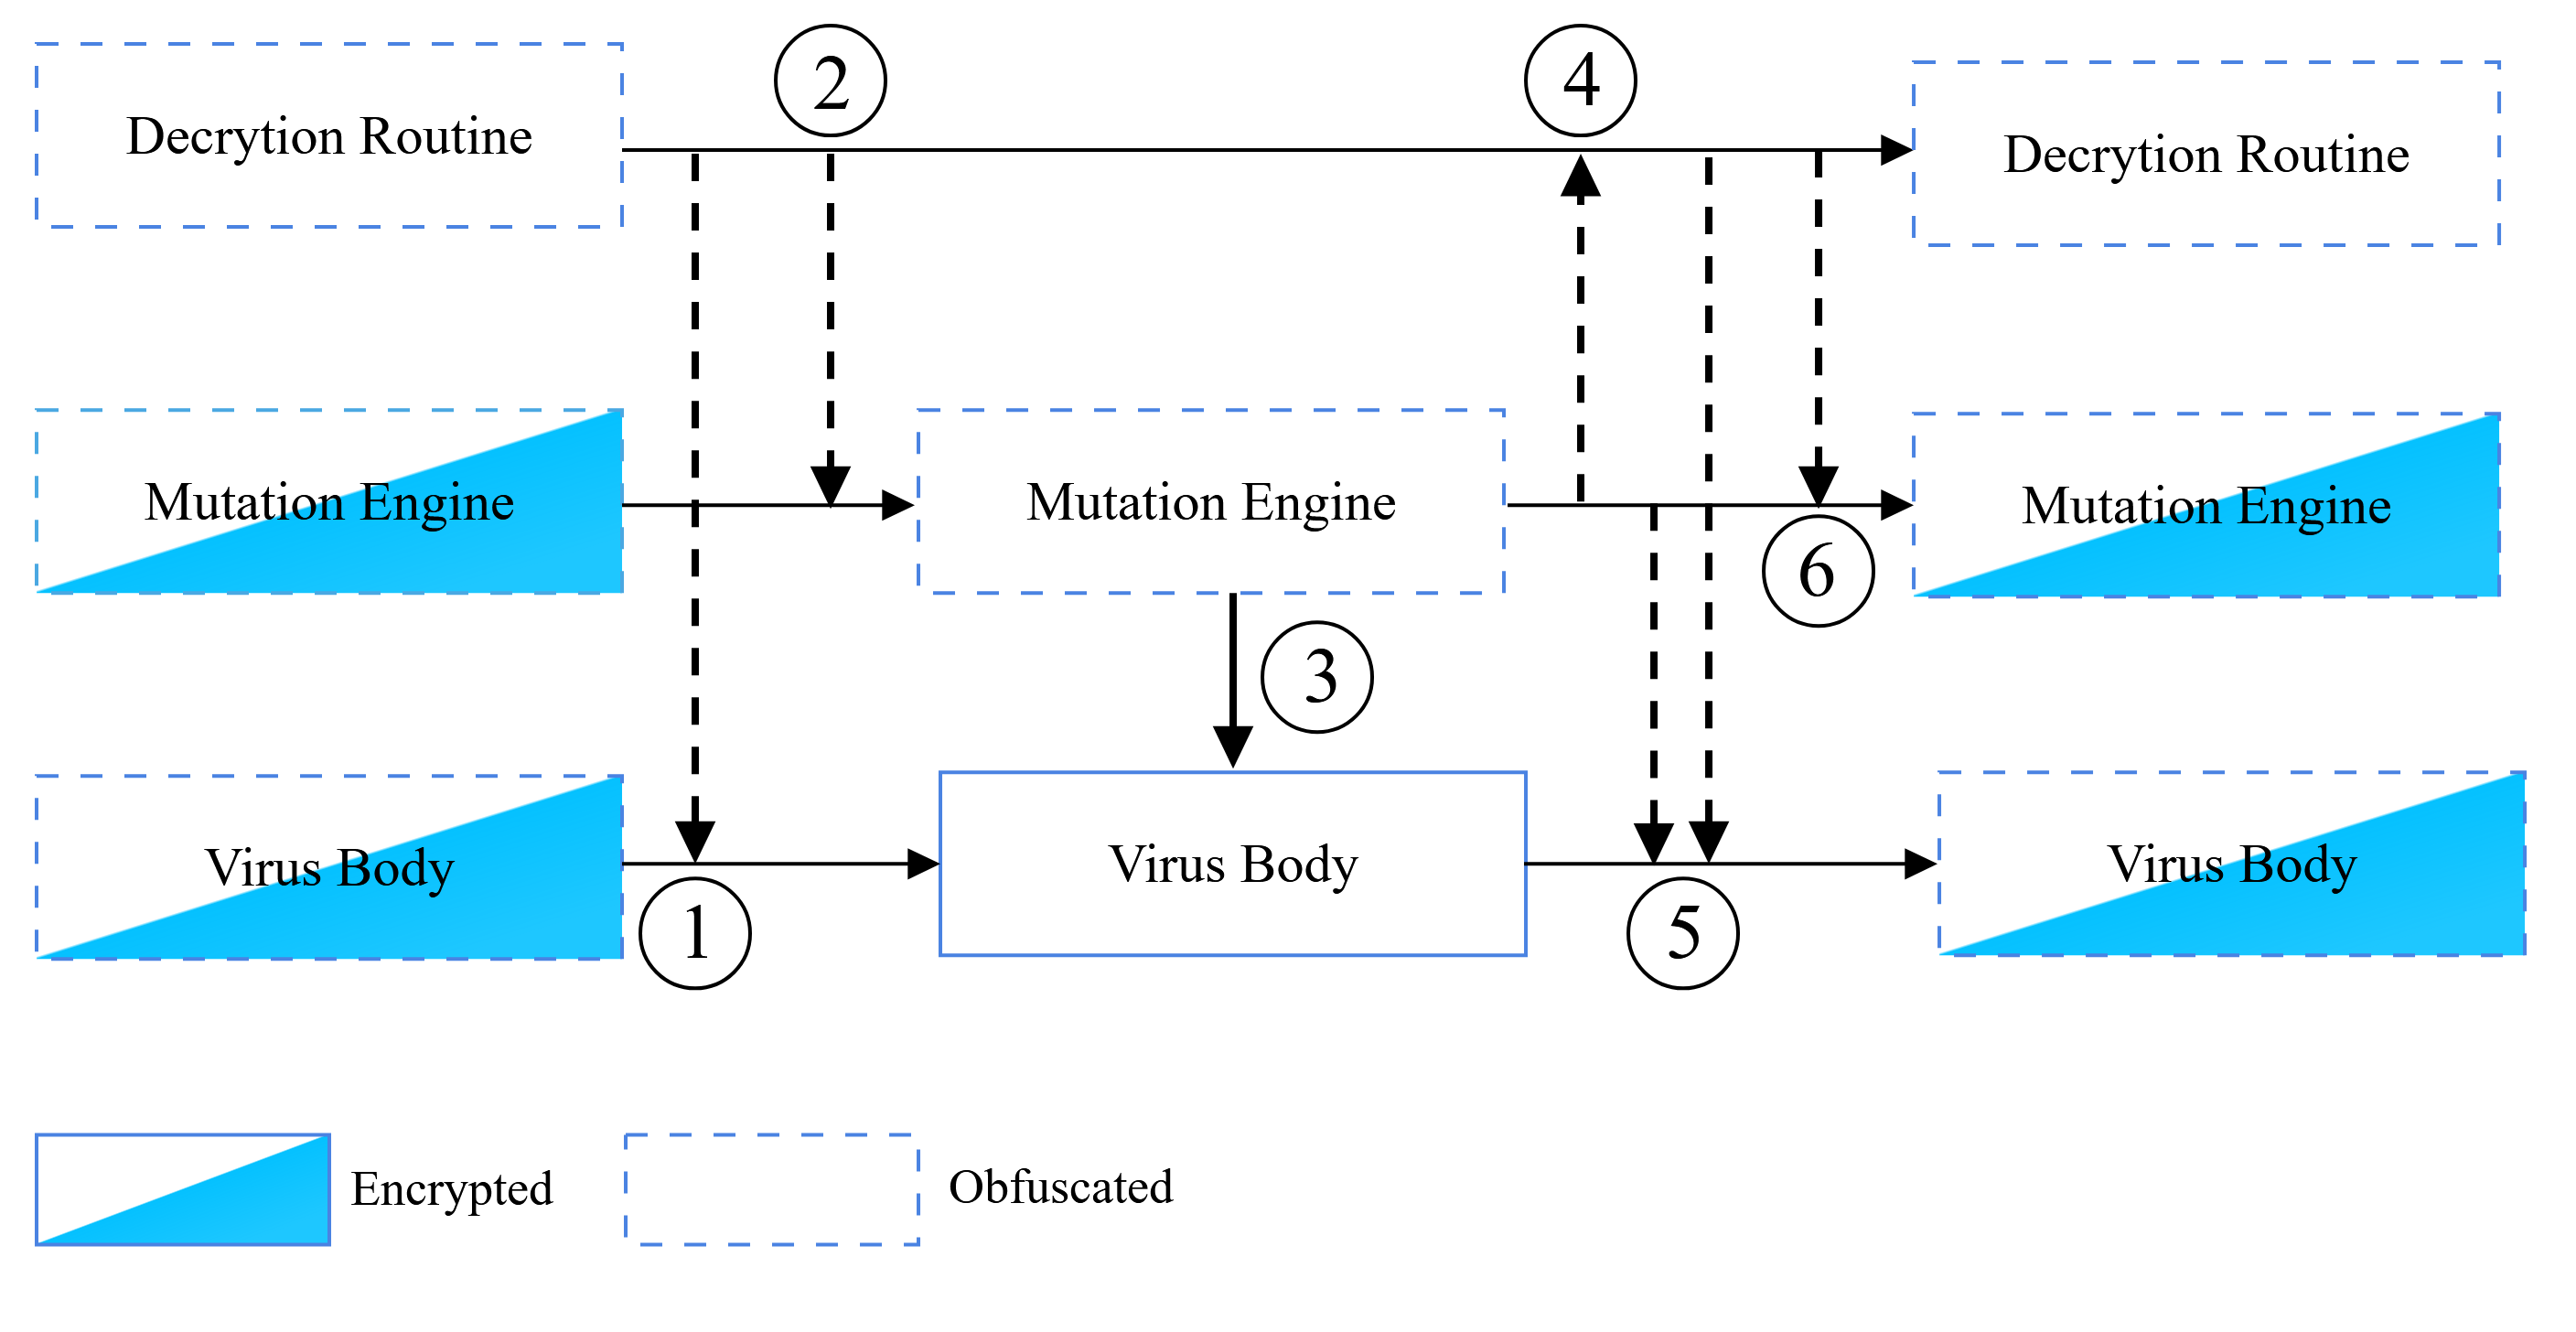
\includegraphics[width=10cm]{images/steps_metamorphic.png}
			\caption{Pasos del Motor Metamórfico para Desencriptar}
		\end{figure}
   	   	
  	\end{frame}
  
   \begin{frame}{Entropía}
   \section{Entropía}
   Claude E. Shannon en \textit{A Mathematical Theory of Communication} desarrolló una fórmula donde, se puede identificar la aleatoriedad o desorden de un sistema, de manera que podamos identificar si una muestra ha sido ofuscada o no. Cuanto más alta sea la probabilidad y sobre todo mayor de \textit{3.75} significa que no ha sido escrito por un humano.
  	\[H(X) = - \sum P (x_i) log P (x_i)\] 
  	
  
  \end{frame}

    
   \begin{frame}{Entropía}
		\begin{figure}[H]
			\centering
			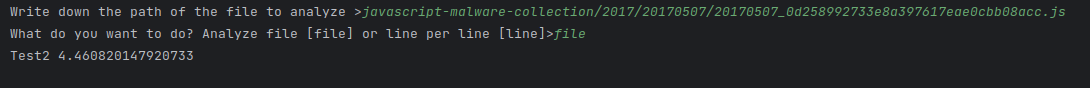
\includegraphics[width=13cm]{images/tool_1.png}
			\caption{Análisis del Fichero Completo}
		\end{figure}
		
		
		\begin{figure}[H]
			\centering
			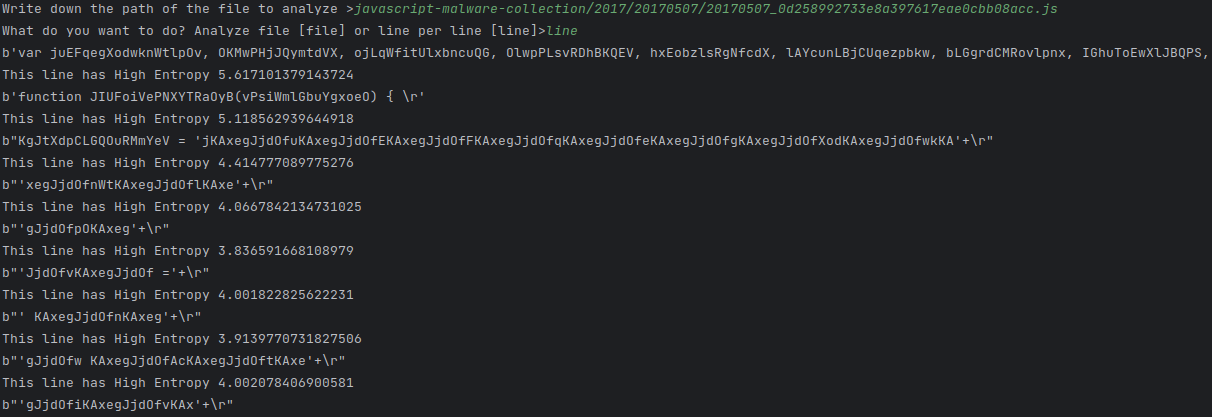
\includegraphics[width=13cm]{images/tool_2.png}
			\caption{Análisis del Fichero por Líneas }
		\end{figure}
    \end{frame}
    
    \begin{frame}{Importancia de las amenazas de JavaScript en Windows}
   	\section{Importancia de las amenazas de JavaScript en Windows}
   	
   	\begin{itemize}
   		\item 40\% de las amenazas, ataques basados en uso de scripts.
   		\item Uso de PowerShell, VBScript  y JavaScript
   		\item JavaScript de Windows cada vez más utilizado, todo el malware se está migrando a JavaScript.
   		\item Desde un dropper destinado a entregar malware adicional hasta partes de malware.
   
   	\end{itemize}
   	
   	\end{frame}
   	\begin{frame}{Importancia de las amenazas de JavaScript en Windows}
   	 Ejemplos de malware:
   	\begin{itemize}
   		\item WJworm. Troyano de Acceso Remoto (RAT), Ataque Denegación de Servicio (DDOS), propagado por adjuntos de email.
   		\item  WSHRat. Migrado de VBS a JavaScript en 2019, Troyano RAT propagado por adjuntos de email.
   		\item STRRAT. Dropper en JavaScript, propagado por archivos adjuntos. Ransomware.
   		\item BlackByte. Ransomware, wrapper en JavaScript
   		\item Carbanak/FIN7. Backdoor en JavaScript para ejecutar comandos.

   	\end{itemize}

   	\end{frame}
   	
	\begin{frame}{Desofuscación de código en JavaScript}
	\section{Desofuscación de código en JavaScript}
	 Las técnicas más utilizadas de ofuscación en el malware que utiliza JavaScript son:
	
	\begin{itemize}
		\item Nos podemos encontrar todo el código en una sola línea.
		\item Uso de funciones con llamada instantánea tipo \textit{(function hello(){})()}
		\item Concatenación de caracteres, conjuntos de caracteres, uso de \textit{parseInt} y \textit{toString} para sustituir un caracter por su valor equivalente.
		\item Llamar a funciones con cadenas de caracteres.
		\item Operadores lógicos equivalentes tipo \textit{+!!false} que es 0
		\item Función \text{eval} con conjuntos de números
		\item Uso de caracteres Unicode, hexadecimal y formato URL
		\item Base64 para ocultar cadenas de caracteres como URLs	
	\end{itemize}
	
	\end{frame}
	
	\begin{frame}{Desofuscación de código en JavaScript}
		\begin{figure}[H]
			\centering
			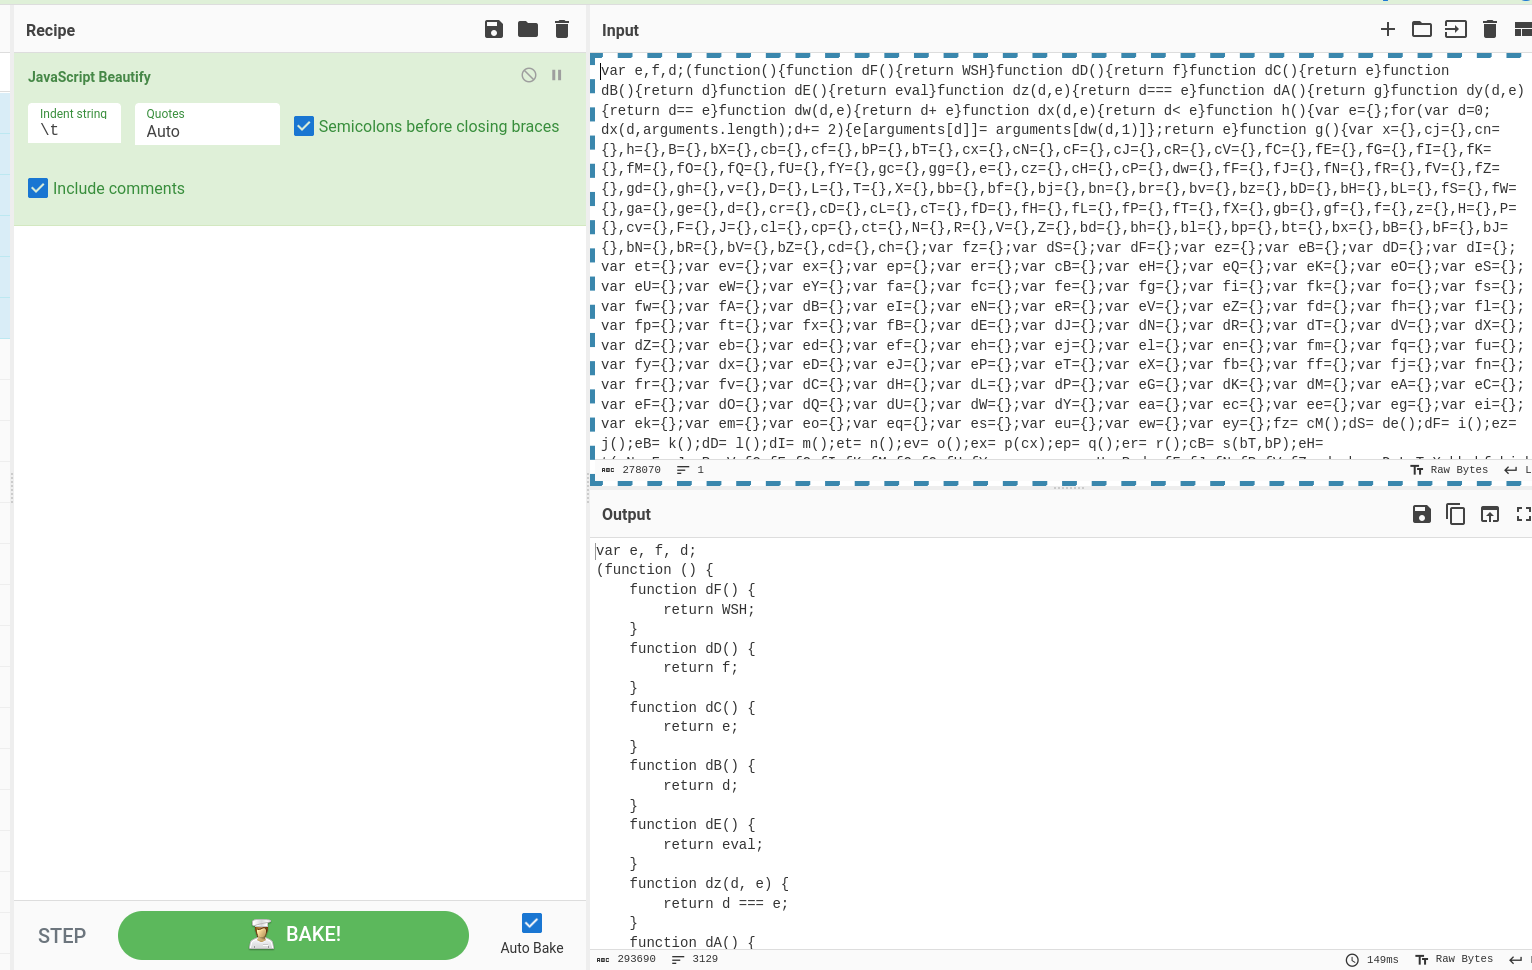
\includegraphics[width=10cm]{images/beautifully.png}
			\caption{CyberChef JavaScript Beautifully}
		\end{figure}
	
	\end{frame}

	
	\begin{frame}{Desofuscación de código en JavaScript}
	\begin{figure}[H]
		\centering
		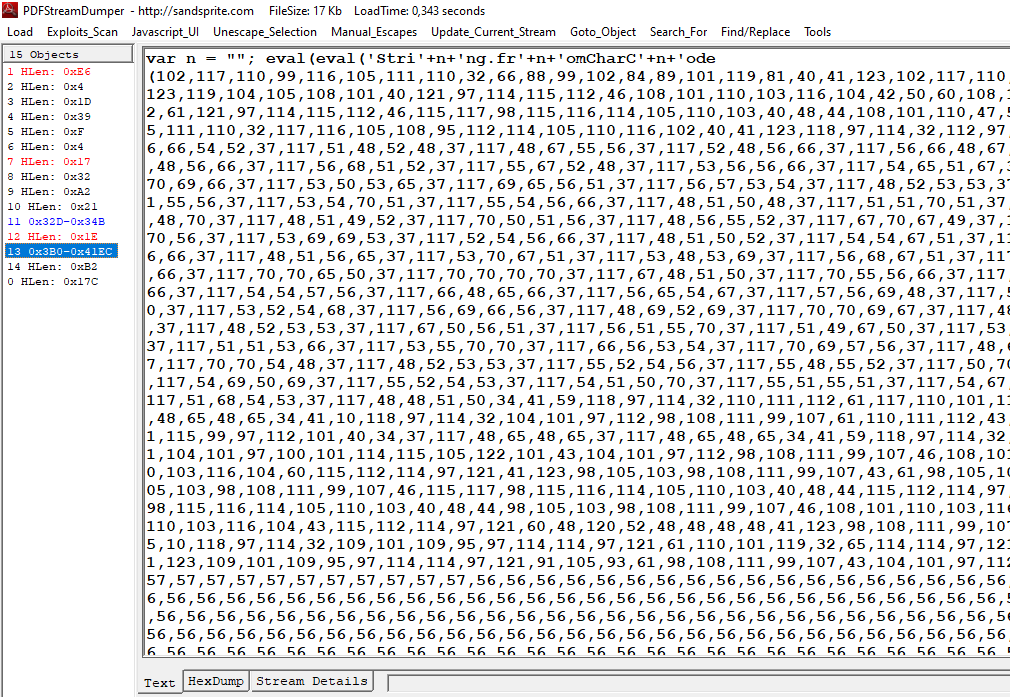
\includegraphics[width=12cm]{images/pdf1.png}
		\caption{Eval + conjunto de enteros}
	\end{figure}
	
	\end{frame}

	
	\begin{frame}{Desofuscación de código en JavaScript}
		
	\begin{figure}[H]
		\centering
		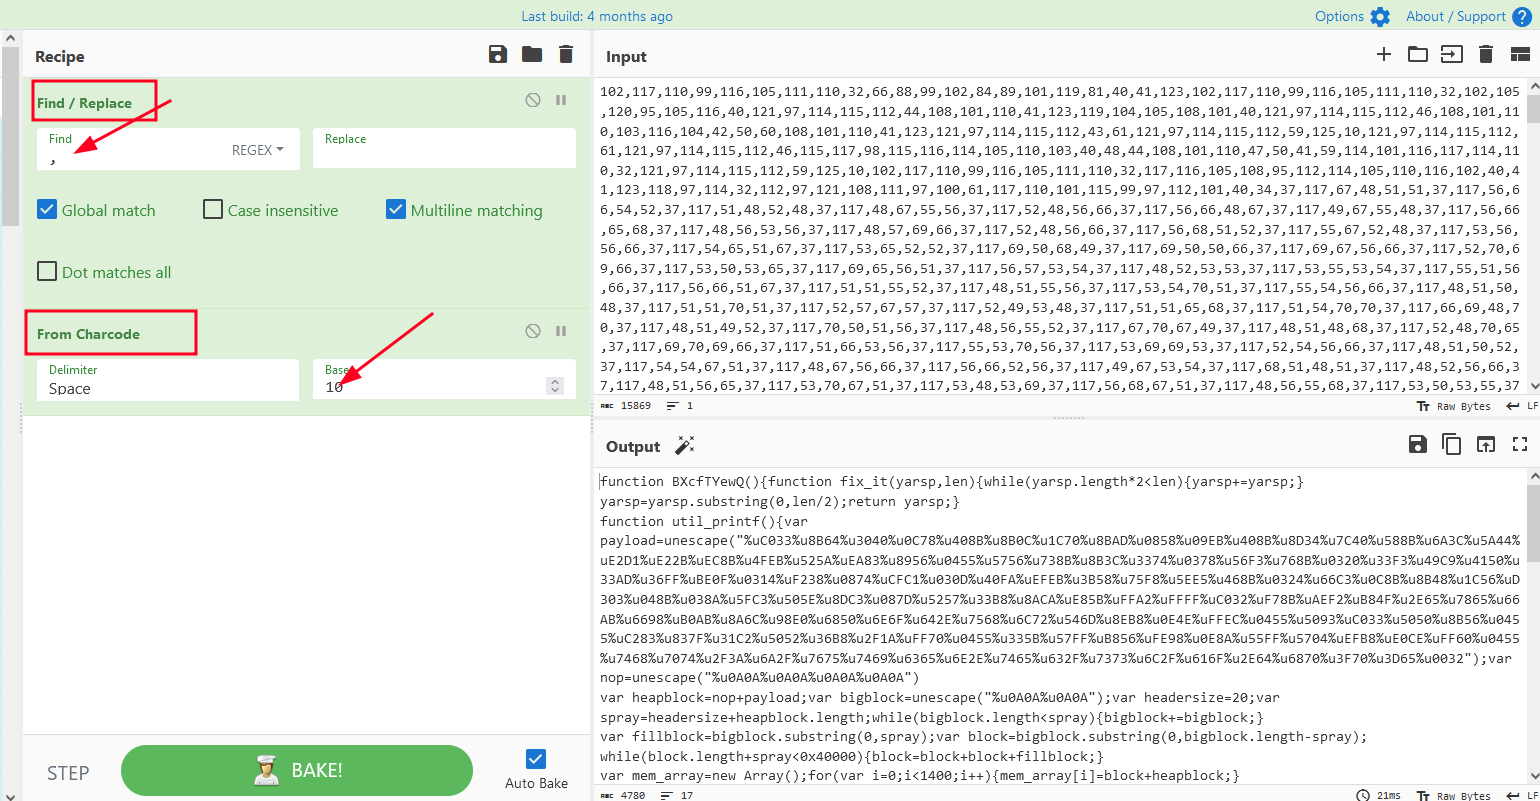
\includegraphics[width=12cm]{images/pdf2.png}
		\caption{Eval + conjunto de enteros}
	\end{figure}
	
	\end{frame}
    
  
  	\begin{frame}{Desofuscación de código en JavaScript}
  		
  		\begin{figure}[H]
  			\centering
  			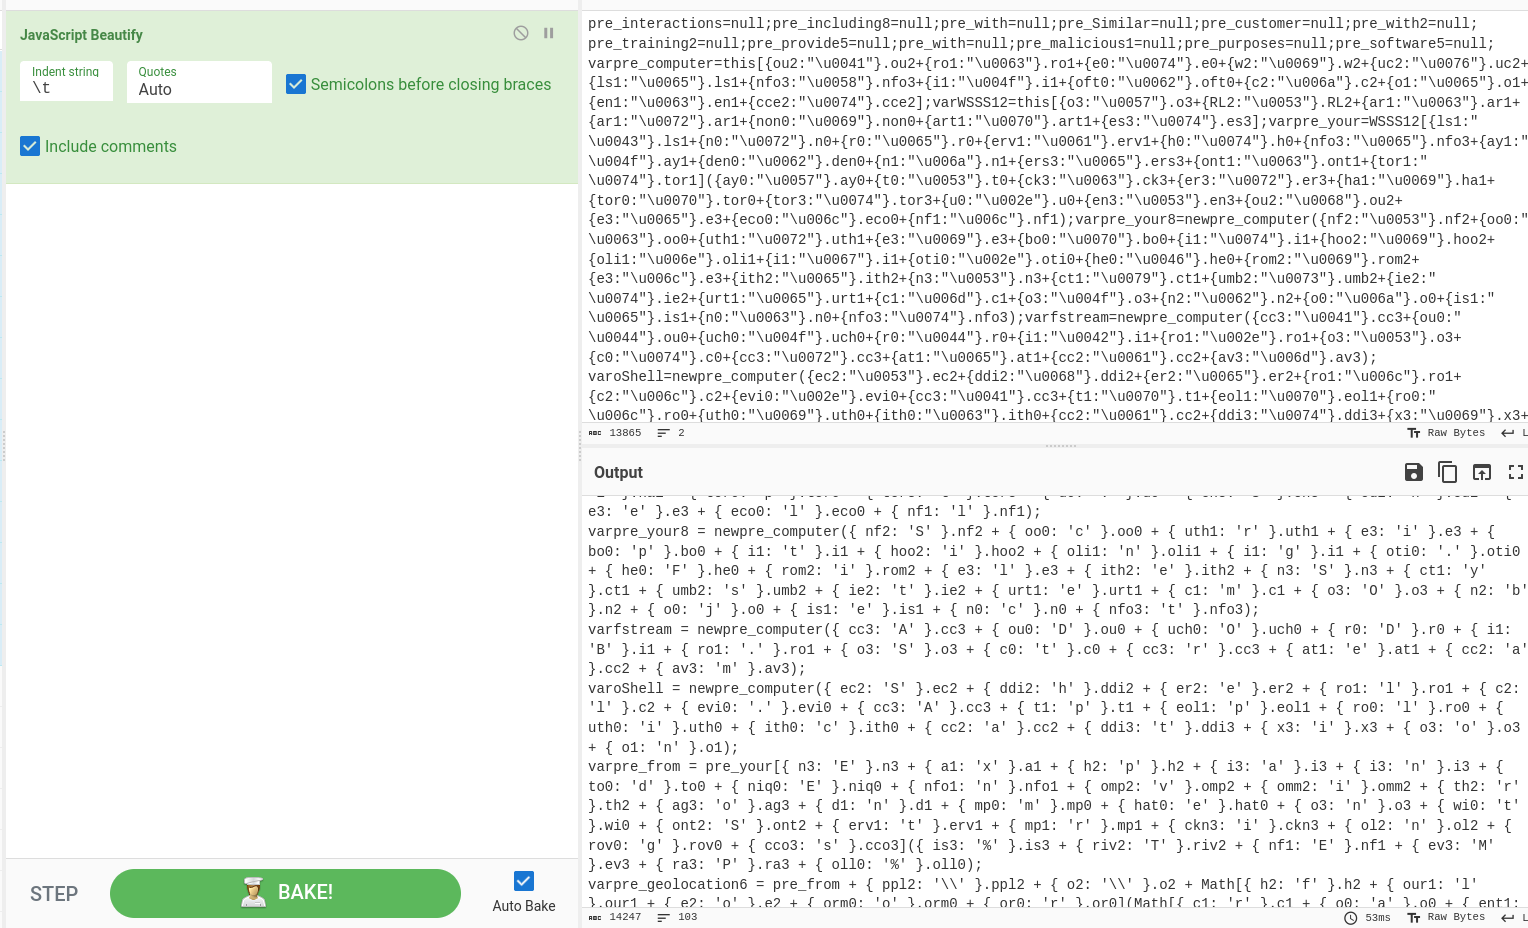
\includegraphics[width=10cm]{images/unicode.png}
  			\caption{Caracteres unicode}
  		\end{figure}
  	\end{frame}
	\begin{frame}{Desofuscación de código en JavaScript}
		
		\begin{figure}[H]
			\centering
			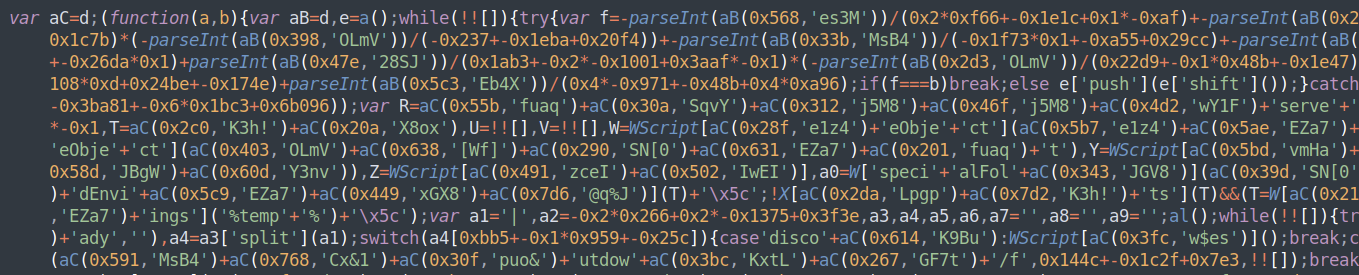
\includegraphics[width=12cm]{images/hexadecimal.png}
			\caption{Caracteres hexadecimales}
		\end{figure}
	\end{frame}
     
   	\begin{frame}{Desofuscación de código en JavaScript}
   		
   		\begin{figure}[H]
   			\centering
   			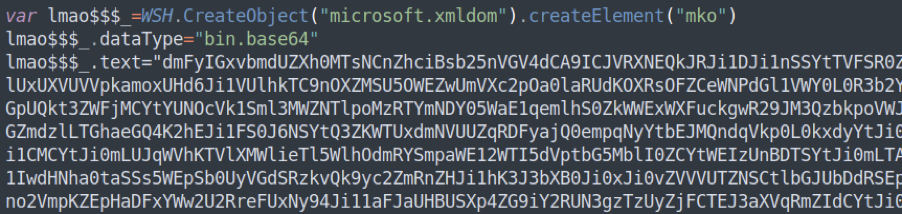
\includegraphics[width=12cm]{images/base64.png}
   			\caption{Caracteres en base64}
   		\end{figure}
   	\end{frame}
      
    
  	\begin{frame}{Freyja Deobfuscation Tool}
  	\section{Freyja Deobfuscation Tool}
  		\href{https://github.com/drkrysSrng/freyja}{@drkrysSrng/freyja}
	\begin{figure}[H]
		\centering
		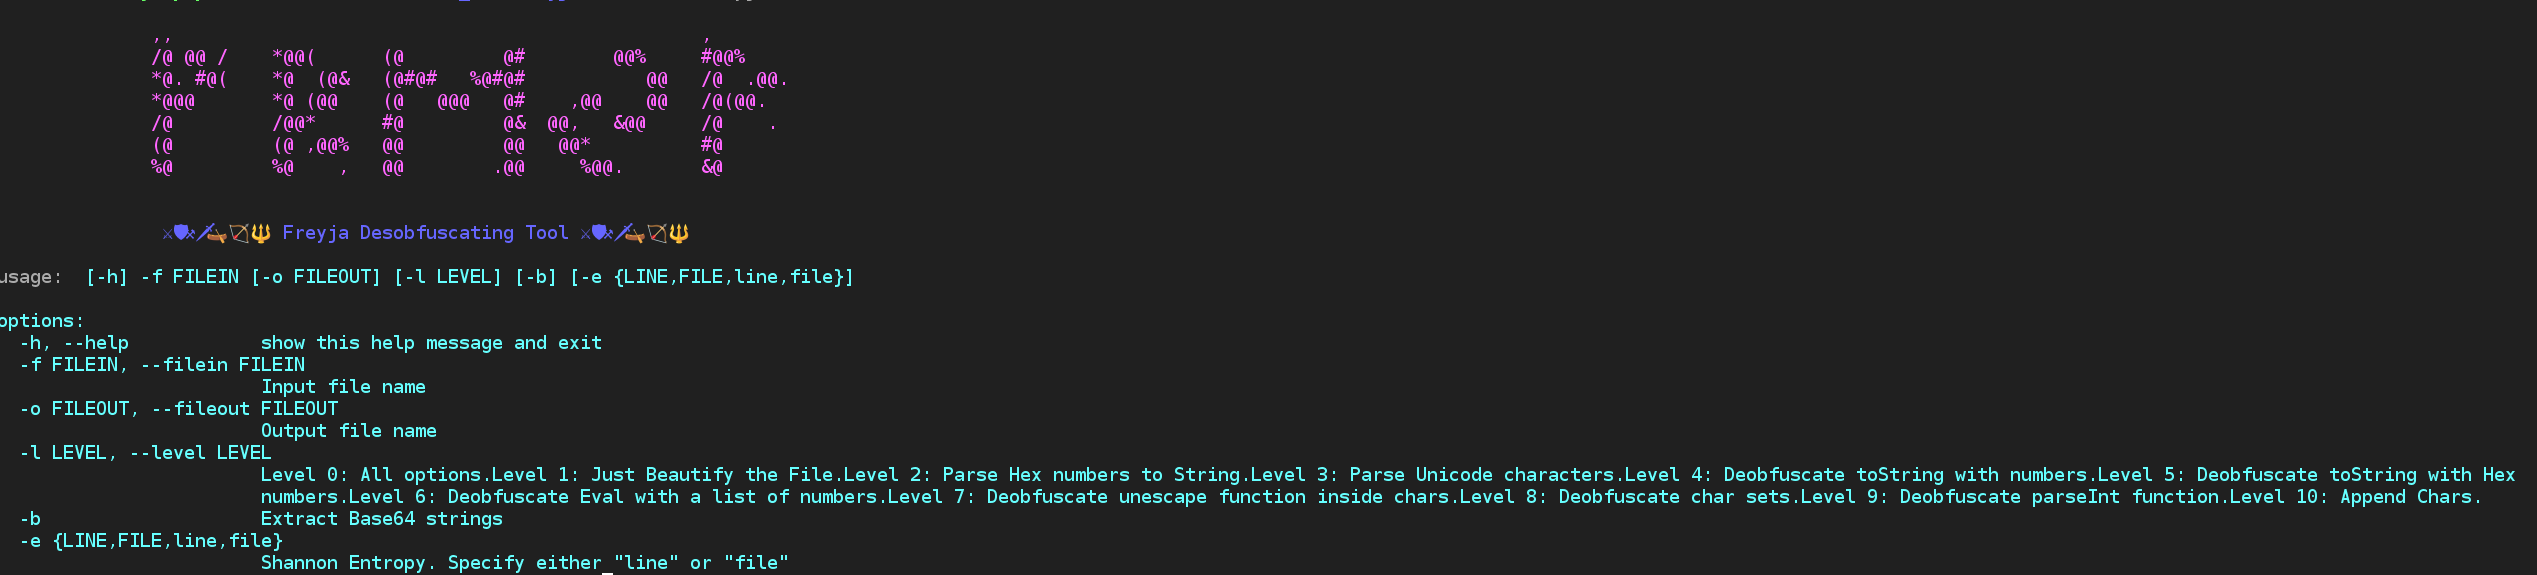
\includegraphics[width=15cm]{images/usage.png}
	\end{figure}
  	
  	\end{frame}
  	\begin{frame}{Funcionamiento}
  	\subsection{Funcionamiento}
	\begin{itemize}
		\item \textit{-f} Fichero a desofuscar.
		\item \textit{-o} Fichero de salida desofuscado.
		\item \textit{-l} Nivel de ofuscación. Le indicamos la técnica que queremos que utilice.
		\begin{itemize}
			\item Nivel 0: Todas las opciones
			\item Nivel 1: Técnica \textit{beautify}, tabular el fichero y darle formato al JavaScript.			
			\item Nivel 2: Parsear los caracteres Hexadecimal a Strings.
			\item Nivel 3: Parsear los caracteres Unicode a Strings.
			\item Nivel 4: Desofuscar la función \textit{toString}.
			\item Nivel 5: Desofuscar la función  \textit{toString} con número hexadecimal.
			\item Nivel 6: Desofuscar la función  \textit{eval} cuando tiene una lista de números.
			\item Nivel 7: Desofuscar la función  \textit{unescape} cuando contiene caracteres.
			\item Nivel 8: Desofuscar conjuntos de caracteres.
			\item Nivel 9: Desofuscar la función  \textit{parseInt}.
			\item Nivel 10: Concatena caracteres aunque estén en varias líneas.
		\end{itemize}
	\end{itemize}
  	\end{frame}
  	
  	\begin{frame}{Funcionamiento}
		\begin{figure}[H]
			\centering
			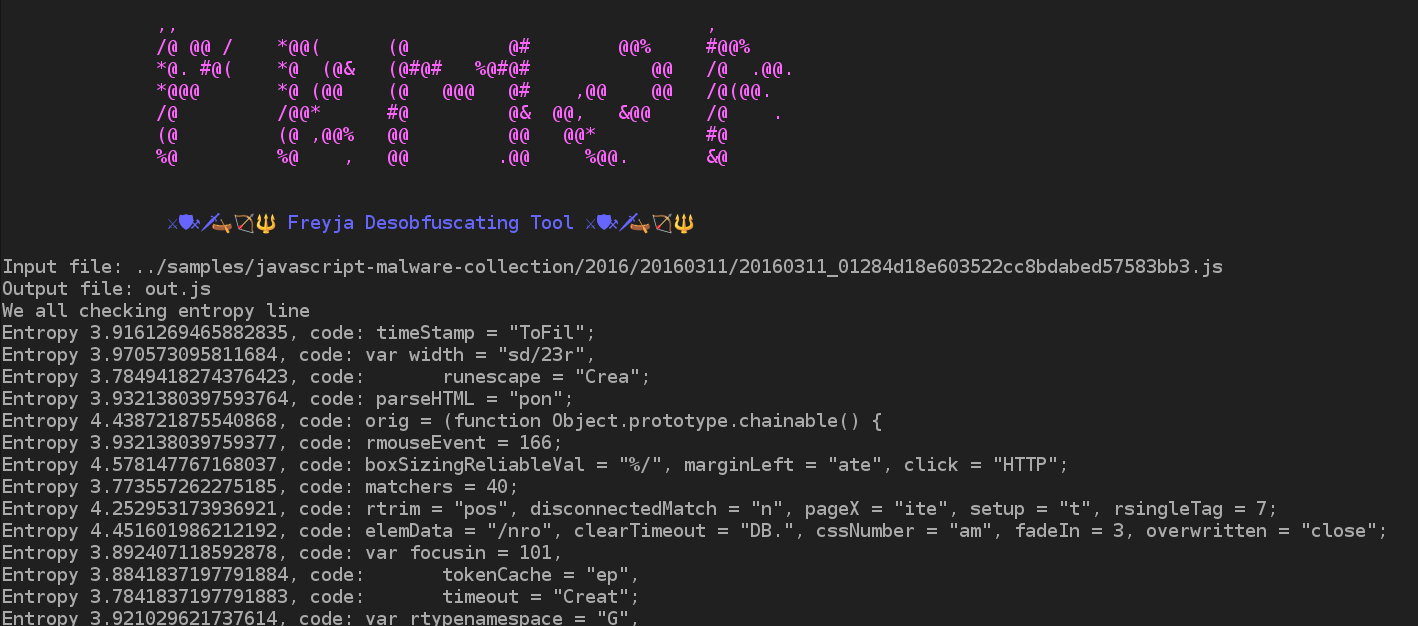
\includegraphics[width=15cm]{images/line_entropy.png}
			\caption{Entropía por líneas}
		\end{figure}
  	\end{frame}
  	\begin{frame}{Funcionamiento}
		\begin{figure}[H]
			\centering
			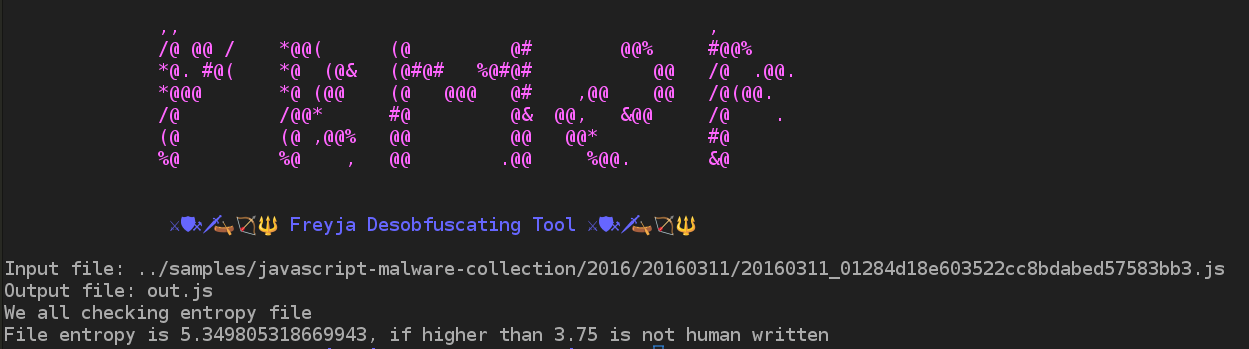
\includegraphics[width=15cm]{images/file_entropy.png}
			\caption{Entropía del fichero completo}
		\end{figure}
  	\end{frame}
  	

  	\begin{frame}{Funcionamiento}
		\begin{figure}[H]
			\centering
			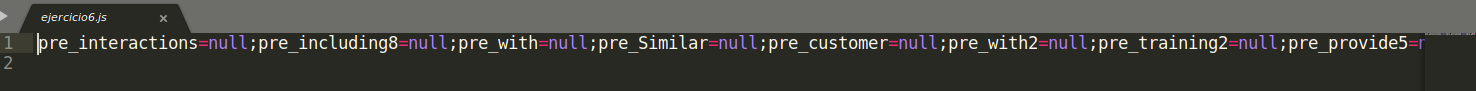
\includegraphics[width=12cm]{images/level1.png}
			\caption{Nivel 1: Beautify} 
		\end{figure}
  	\end{frame}
  	\begin{frame}{Funcionamiento}
		\begin{figure}[H]
			\centering
			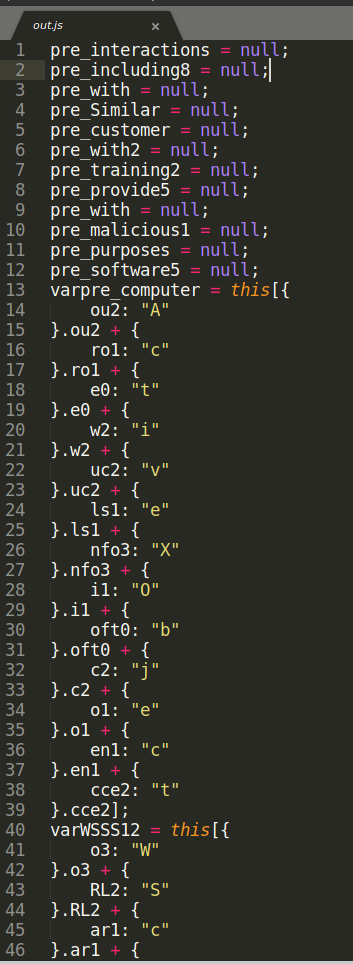
\includegraphics[width=3cm]{images/level1_after.png}
		\end{figure}
  	\end{frame}
  	\begin{frame}{Funcionamiento}
		\begin{figure}[H]
			\centering
			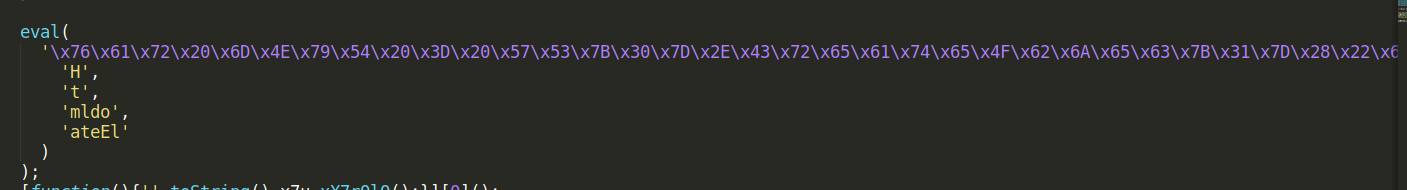
\includegraphics[width=12cm]{images/level2.png}
			\caption{Nivel 2: Hexadecimal Ofuscado} 
		\end{figure}
		
		\begin{figure}[H]
			\centering
			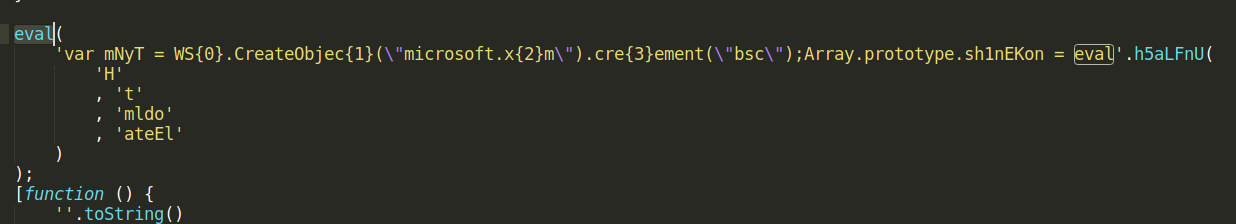
\includegraphics[width=12cm]{images/level2_after.png}
			\caption{Nivel 2: Hexadecimal Desofuscado} 
		\end{figure}
  	\end{frame}
  	
  	\begin{frame}{Funcionamiento}
		\begin{figure}[H]
			\centering
			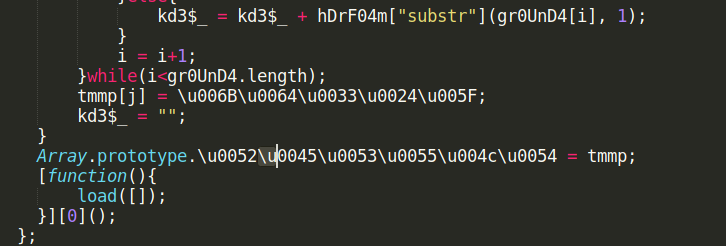
\includegraphics[width=8cm]{images/level3.png}
			\caption{Nivel 3: Unicode} 
		\end{figure}
		
		\begin{figure}[H]
			\centering
			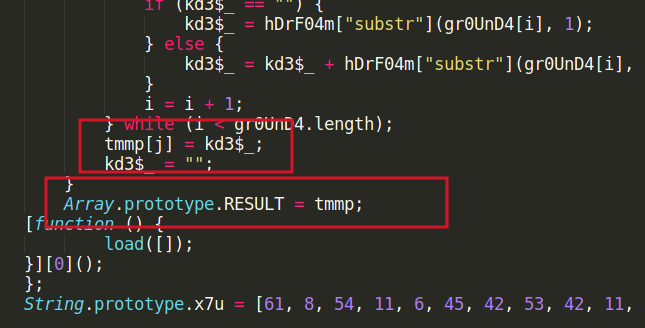
\includegraphics[width=8cm]{images/level3_after.png}
		\end{figure}
  	\end{frame}
  	\begin{frame}{Funcionamiento}
		\begin{figure}[H]
			\centering
			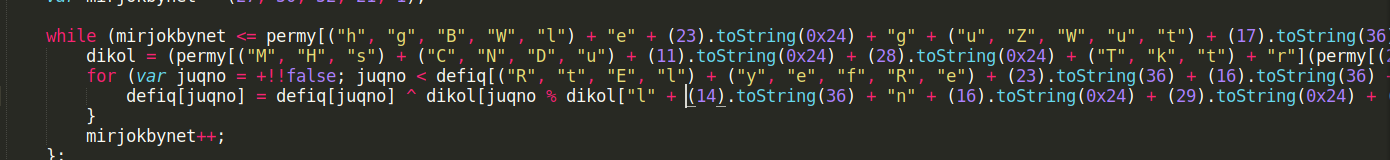
\includegraphics[width=15cm]{images/level4.png}
			\caption{Nivel 4 y 5: toString Ofuscado} 
		\end{figure}
		
		\begin{figure}[H]
			\centering
			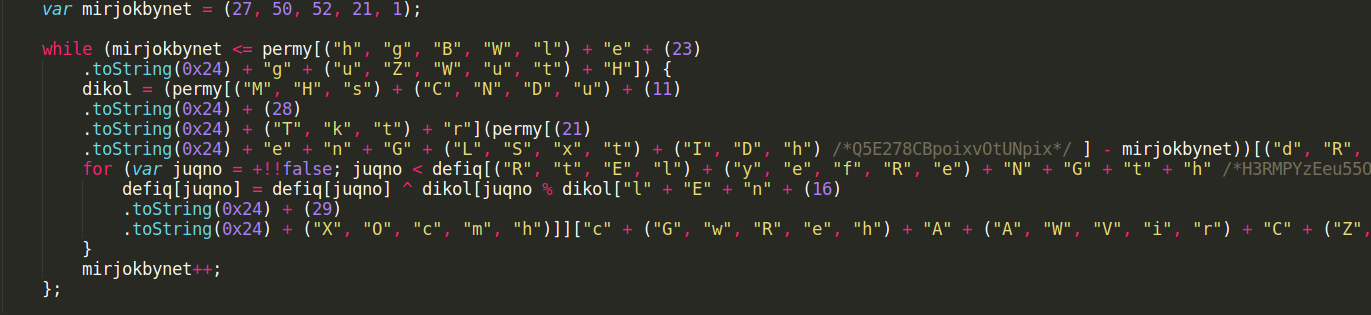
\includegraphics[width=15cm]{images/level4_after.png}
			\caption{Nivel 4: toString Desofuscado} 
		\end{figure}
  	\end{frame}
  	\begin{frame}{Funcionamiento}
		\begin{figure}[H]
			\centering
			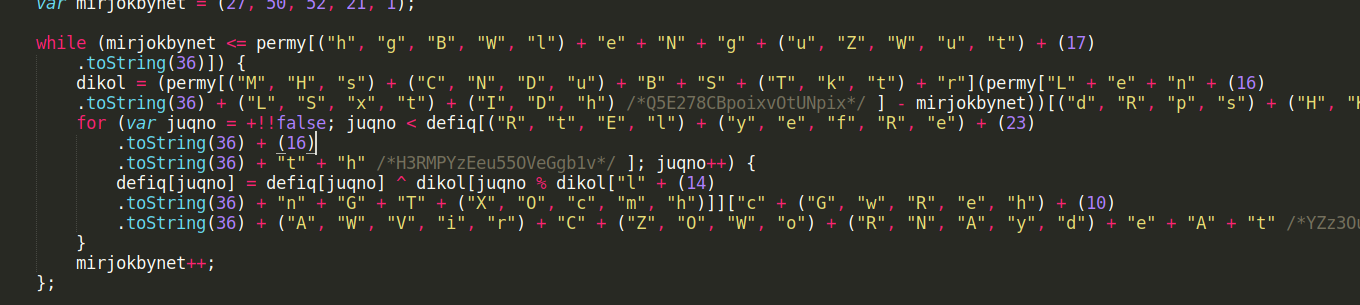
\includegraphics[width=15cm]{images/level5_after.png}
			\caption{Nivel 4: toString Hex Desofuscado} 
		\end{figure}
  	\end{frame}
  	
  	\begin{frame}{Funcionamiento}
	\begin{figure}[H]
		\centering
		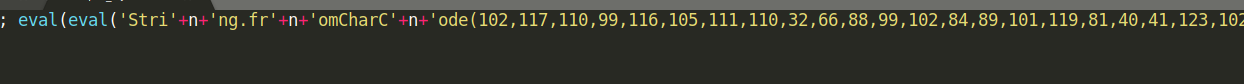
\includegraphics[width=15cm]{images/level6.png}
		\caption{Nivel 6: Eval Ofuscado} 
	\end{figure}
	
	\begin{figure}[H]
		\centering
		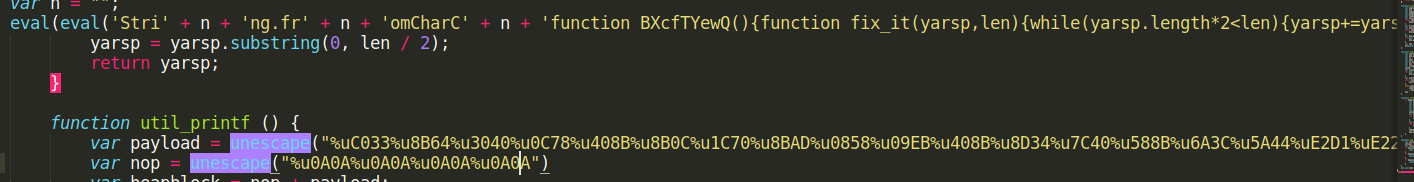
\includegraphics[width=15cm]{images/level6_after.png}
		\caption{Nivel 6: Eval Desofuscado} 
	\end{figure}
  	\end{frame}
  	
  	\begin{frame}{Funcionamiento}
	\begin{figure}[H]
		\centering
		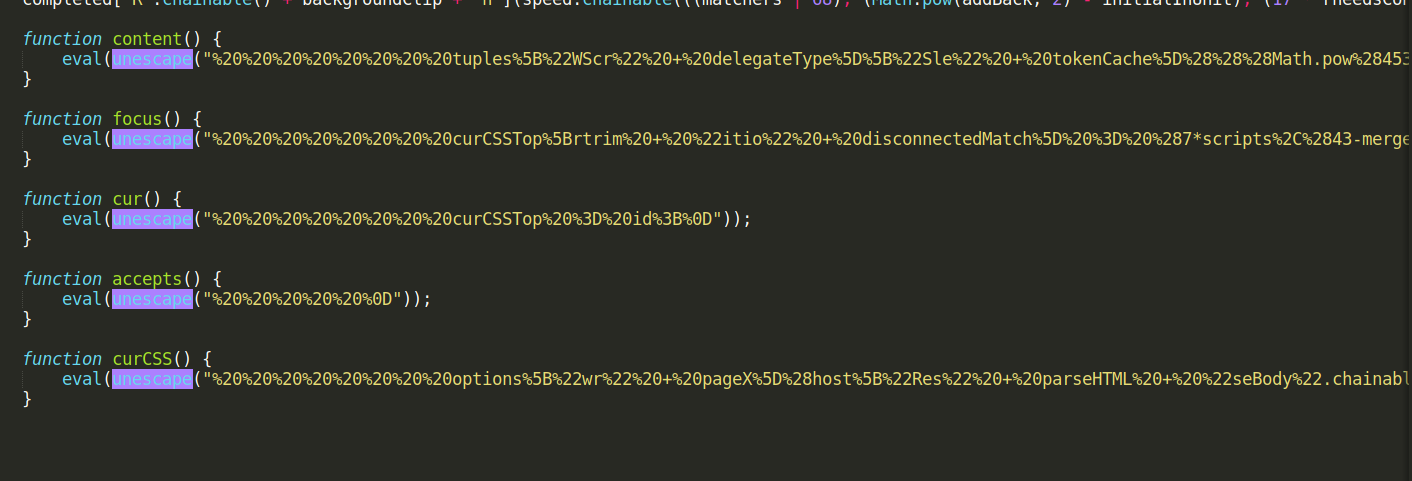
\includegraphics[width=12cm]{images/level7.png}
		\caption{Nivel 7: unescape } 
	\end{figure}
	
	\begin{figure}[H]
		\centering
		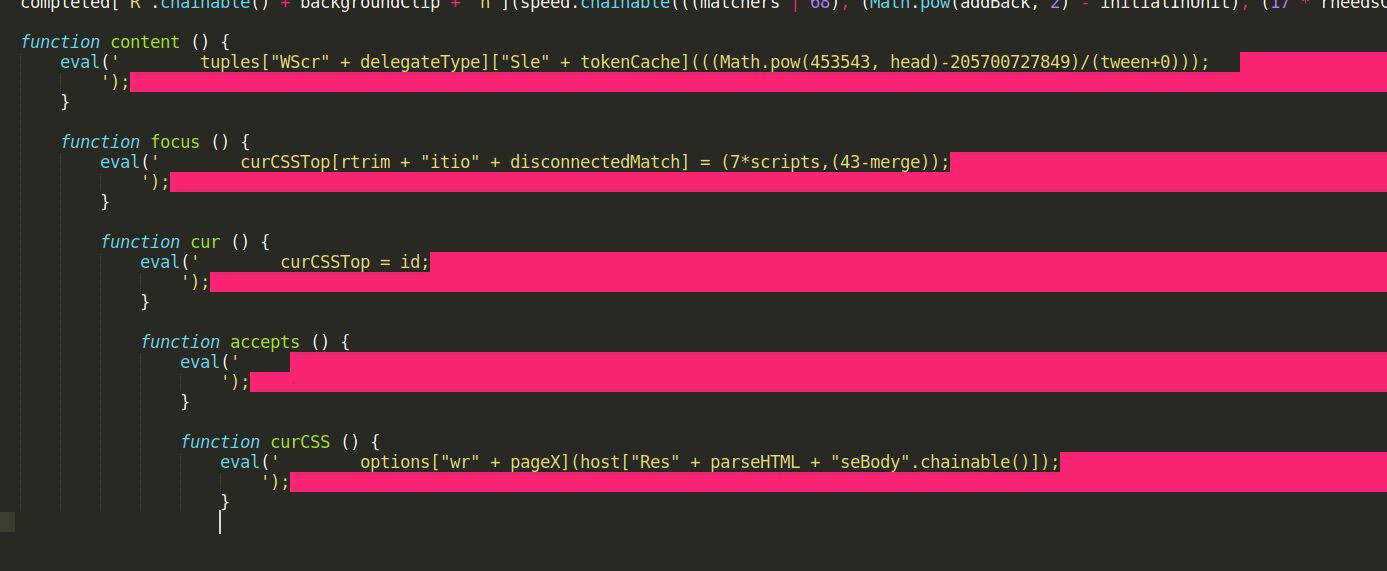
\includegraphics[width=12cm]{images/level7_after.png}
	\end{figure}
  	\end{frame}
  	
  	\begin{frame}{Funcionamiento}
	\begin{figure}[H]
		\centering
		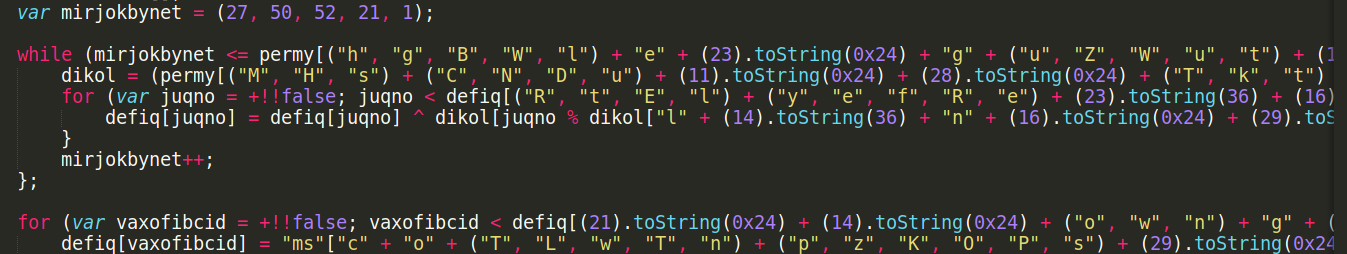
\includegraphics[width=12cm]{images/level8.png}
		\caption{Nivel 8: Conjuntos de caracteres} 
	\end{figure}
	
	\begin{figure}[H]
		\centering
		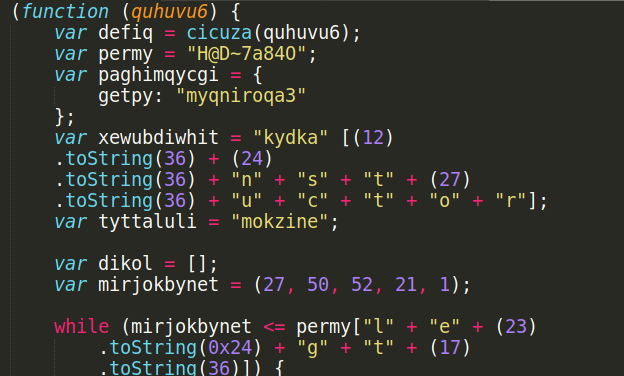
\includegraphics[width=8cm]{images/level8_after.png}
	\end{figure}
  	\end{frame}
  	\begin{frame}{Funcionamiento}
	\begin{figure}[H]
		\centering
		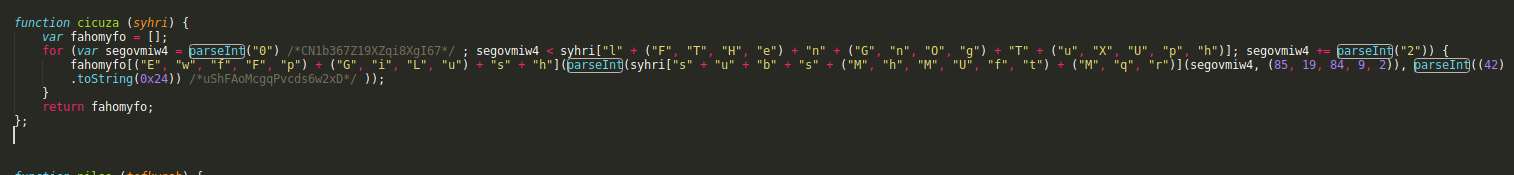
\includegraphics[width=15cm]{images/level9.png}
		\caption{Nivel 9: parseInt Ofuscado} 
	\end{figure}
	
	\begin{figure}[H]
		\centering
		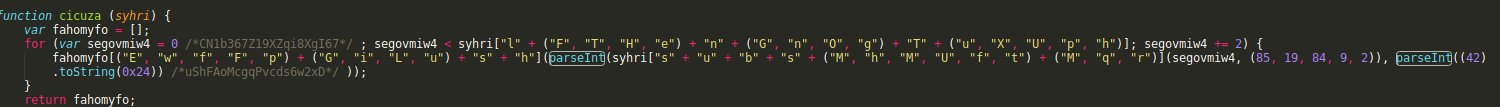
\includegraphics[width=15cm]{images/level9_after.png}
		\caption{Nivel 9: parseInt Desofuscado} 
	\end{figure}
  	\end{frame}
  	\begin{frame}{Funcionamiento}
	\begin{figure}[H]
		\centering
		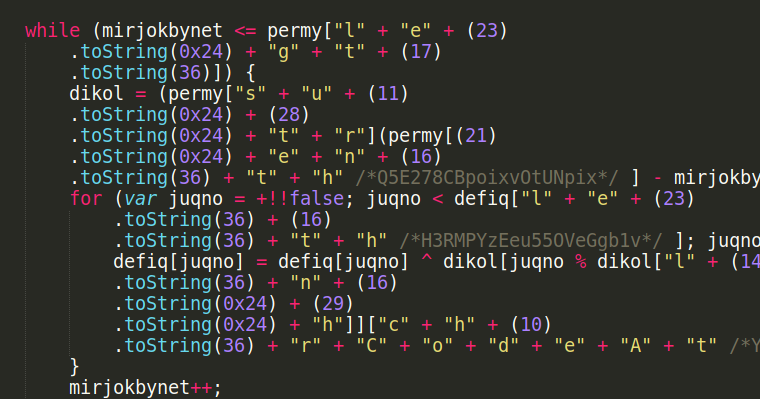
\includegraphics[width=10cm]{images/level10.png}
		\caption{Nivel 10: Concatenación Ofuscada} 
	\end{figure}
	
  	\end{frame}
  	\begin{frame}{Funcionamiento}
	\begin{figure}[H]
		\centering
		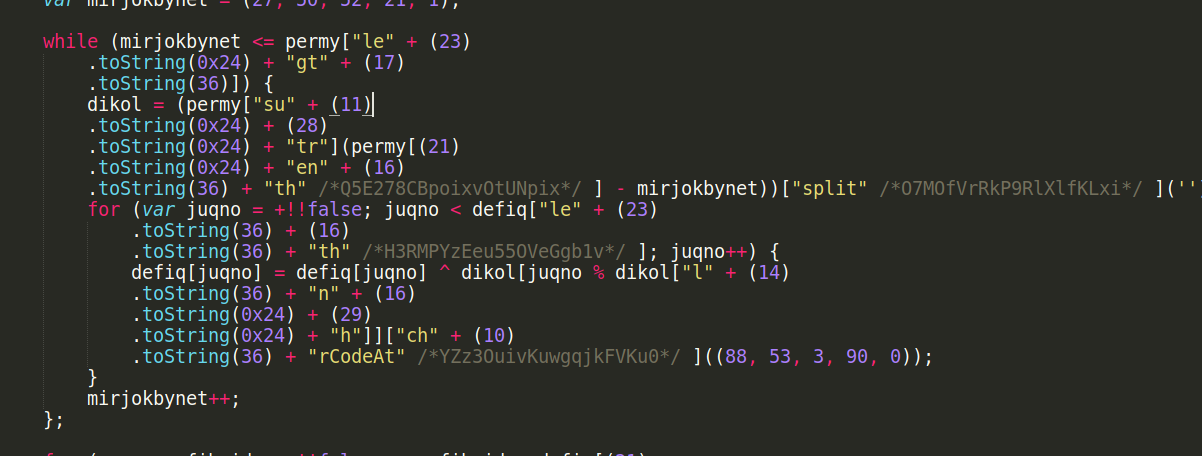
\includegraphics[width=10cm]{images/level10_after.png}
		\caption{Nivel 10: Concatenación Desofuscada} 
	\end{figure}
  	\end{frame}
  	\begin{frame}{Funcionamiento}
	\begin{figure}[H]
		\centering
		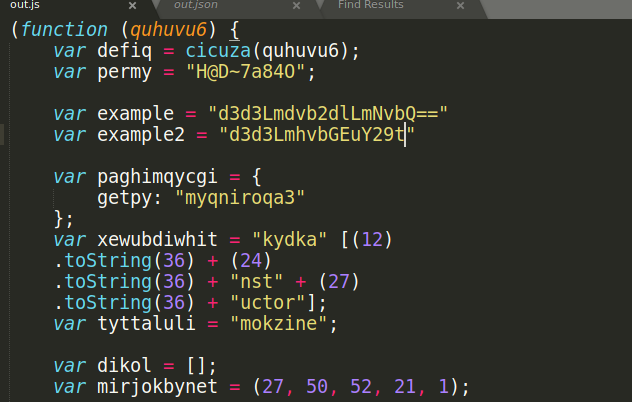
\includegraphics[width=10cm]{images/base64_before.png}
		\caption{Búsqueda de Base64 Ofuscada} 
	\end{figure}
	
  	\end{frame}
  	\begin{frame}{Funcionamiento}
	\begin{figure}[H]
		\centering
		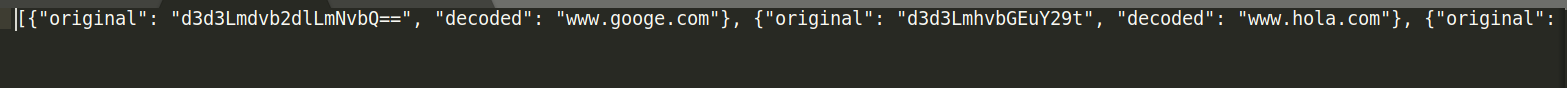
\includegraphics[width=15cm]{images/base64_after.png}
		\caption{Búsqueda de Base64 Desofuscada} 
	\end{figure}
  	\end{frame}

\end{document}